% =============================================
% CHAPITRE 4 — INCRÉMENT 2
% =============================================

\chapter{Spécification des Besoins et Architecture}
\label{chap:specification-architecture}
\vspace{1em}
\noindent\textbf{\large Sommaire}
\vspace{0.5em}
\localtableofcontents
\clearpage

Ce chapitre pose les fondements de la phase de réalisation du système eKYC. Il commence par identifier les acteurs impliqués et formaliser l'ensemble des besoins fonctionnels et non fonctionnels de la plateforme, puis décrit l'architecture logique et physique retenue pour y répondre. L'ensemble est consolidé par un diagramme de cas d'utilisation global et la description détaillée de chaque interaction, constituant ainsi le référentiel de conception sur lequel s'appuient les chapitres de réalisation suivants.

%=============================================================
\section{Spécification des besoins}
\label{sec:specification-besoins}
%=============================================================

\subsection{Identification des acteurs}
\label{subsec:identification-acteurs}

Le système eKYC développé dans ce projet met en interaction plusieurs acteurs aux responsabilités bien distinctes. Le Tableau~\ref{tab:acteurs_pfe} présente chaque acteur, sa nature et son rôle au sein de la plateforme.

\renewcommand{\arraystretch}{1.5}
\begin{longtable}{|>{\bfseries}p{3.8cm}|p{10.2cm}|}
  \hline
  \rowcolor{bleu_clair!20}
  \textbf{Acteur} & \textbf{Rôle et responsabilités} \\
  \hline
  \endfirsthead
  \hline
  \rowcolor{bleu_clair!20}
  \textbf{Acteur} & \textbf{Rôle et responsabilités} \\
  \hline
  \endhead
    Client & 
      Particulier souhaitant ouvrir un compte bancaire. Interagit exclusivement avec l'interface client, accessible sur mobile et navigateur web. Soumet ses documents d'identité, peut corriger les données extraites et réalise la capture biométrique. \\
    \hline
    Analyste KYC & 
      Agent opérationnel de la BTE chargé d'examiner les dossiers traités par le système IA. Consulte les données extraites, les résultats du filtrage AML (\textit{Anti-Money Laundering} / Lutte contre le blanchiment d'argent) et le score de risque, puis prend la décision finale de validation, de rejet ou de demande de complément. \\
    \hline
    Administrateur & 
      Profil à droits étendus qui possède les mêmes fonctionnalités que l'analyste KYC et le responsable qualité du système IA. Consulte le journal d'audit dans son intégralité. \\
    \hline
    Responsable qualité IA & 
      Profil technique chargé de surveiller en continu les performances des modèles d'intelligence artificielle. Consulte les indicateurs de qualité par type de document et par modèle. N'accède à aucune donnée personnelle du client. \\
    \hline
  
  \caption{Acteurs et périmètres d'action du système eKYC}
  \label{tab:acteurs_pfe}
\end{longtable}

\subsection{Besoins fonctionnels}
\label{subsec:besoins-fonctionnels}

Les exigences fonctionnelles définissent les fonctionnalités clés que le système doit fournir pour satisfaire les besoins des utilisateurs.

\paragraph*{S'inscrire}
\begin{itemize}
  \item Créer un compte sur l'application (inscription classique).
\end{itemize}
\paragraph*{S'authentifier}
\begin{itemize} 
  \item Se connecter à la plateforme avec ses identifiants. 
\end{itemize}

\paragraph*{Soumettre et suivre un dossier KYC}
\begin{itemize}
  \item Initier un dossier KYC et choisir le type de document à soumettre (CIN ou passeport).
  \item Capturer son document guidé par un retour visuel en temps réel~; le système détecte automatiquement la présence, le type et la qualité du document via YOLOv8n avant de déclencher la capture.
  \item Consulter et peut corriger les informations extraites automatiquement par le pipeline OCR (YOLOv11m + PaddleOCR) avant soumission finale.
  \item Capturer un selfie biométrique avec un retour visuel en temps réel pour garantir un cadrage conforme au format requis.
  \item Suivre l'état de son dossier .
\end{itemize}

\paragraph*{Demander des services bancaires}

\noindent Une fois son dossier KYC approuvé et son compte bancaire courant ouvert, le client peut :

\begin{itemize}
  \item Soumettre une demande de carte bancaire.
  \item Soumettre une demande de chéquier.
  \item Soumettre une demande de crédit avec le document justificatif requis (attestation de salaire).
  \item Suivre l'état de ses demandes en cours.
\end{itemize}

\paragraph*{Traiter les dossiers KYC}
\begin{itemize}
  \item Consulter la file de traitement des dossiers en attente.
  \item Accéder au détail d'un dossier : données extraites, score de risque, résultat de la comparaison biométrique et alertes AML.
  \item Valider un dossier si les informations sont correctes et le score satisfaisant.
  \item Corriger manuellement un champ extrait erroné avant validation.
  \item Rejeter un dossier en documentant obligatoirement le motif de refus.
  \item demander des informations complémentaires au client en précisant les pièces manquantes ou les corrections à apporter.
\end{itemize}

\paragraph*{Administrer et surveiller la plateforme}
\begin{itemize}
  \item Consulter le registre global de tous les dossiers, tous statuts confondus.
  \item Consulter le journal d'audit immuable de toutes les actions effectuées.
  \item Consulter les indicateurs de performance des modèles IA .
 
\end{itemize}

\bigskip
\noindent L'analyse des besoins révèle que le système eKYC combine deux natures de travail complémentaires : un pipeline IA qui exige une phase de recherche, d'entraînement et de validation avant tout déploiement, et une plateforme applicative dont la réalisation dépend directement des résultats de ce pipeline. Cette interdépendance justifie l'adoption d'un \textbf{modèle de développement incrémental en deux incréments} : le premier consacré à la conception et à la validation du module IA, le second à la réalisation de la plateforme.

\subsection{Besoins non fonctionnels}
\label{subsec:besoins-non-fonctionnels}

Les besoins non fonctionnels définissent les caractéristiques essentielles que doit respecter le système, indépendamment des fonctionnalités métier.

\begin{description}[style=nextline, leftmargin=0pt, labelwidth=!, font=\bfseries\color{black}]

  \item[Sécurité]
  Bien que le cadre de ce projet académique n'impose pas de contraintes de sécurité formelles, nous avons fait le choix d'intégrer des mécanismes de sécurité qui se rapprochent au maximum des standards appliqués en environnement bancaire réel. La plateforme manipule des données d'identité sensibles comme les numéros de CIN, les photos de documents et les selfies, ce qui nous a guidés vers l'adoption de bonnes pratiques dès la conception. L'authentification repose sur des tokens JWT dont la durée de validité est limitée à 60 minutes, les mots de passe sont stockés sous forme hachée avec l'algorithme bcrypt, et les tokens sont révoqués immédiatement à la déconnexion. Les agents et administrateurs disposent d'un circuit d'authentification distinct des clients. Une double authentification est mise en place pour les actions critiques : toute décision sur un dossier nécessite une confirmation du mot de passe avant d'être enregistrée. Toutes les actions sensibles comme la connexion, la décision sur un dossier et la modification de paramètres sont tracées dans un journal d'audit horodaté et non modifiable.
  \item[Confidentialité des données]
  Dans le cadre de ce projet, l'ensemble de la plateforme est déployé en environnement local, simulant les conditions réelles d'un système bancaire où toutes les données restent confinées à l'infrastructure interne de la banque et ne transitent jamais vers l'extérieur. Cette approche reproduit le principe de souveraineté des données qu'une banque applique en production : les photos de documents, les selfies et les données d'identité des clients ne quittent jamais le périmètre du système. Les images sont stockées sur un serveur de fichiers local, et chaque composant y accède directement via une adresse interne sans exposition vers un réseau externe. Les résultats OCR contenant les données d'identité sont conservés temporairement côté client, puis transmis en une seule requête au backend lors de la soumission finale du dossier.
  \item[Conformité réglementaire]
  La plateforme eKYC a été conçue en conformité avec la \textbf{circulaire aux banques n°2025-06 du 28 février 2025} de la Banque Centrale de Tunisie, relative aux règles minimales régissant l'enrôlement électronique des clients~\cite{bct2025circ06}. Conformément aux exigences de cette circulaire, la plateforme met en oeuvre un processus d'identification électronique complet : collecte et vérification des documents d'identité du client, confirmation de la présence réelle du client par reconnaissance faciale (Article 6), filtrage et profilage du risque de chaque client (Article 7), et génération automatique d'une fiche d'identification KYC à l'issue du parcours (Article 8). La plateforme respecte également l'exigence de vigilance proportionnelle au profil de risque (Article 3) en attribuant à chaque dossier un niveau de risque (faible, moyen, élevé ou critique) qui détermine la décision de validation ou de revue manuelle par un agent.

  \item[Performance]
  Le système est conçu pour minimiser le temps de traitement perçu par le client à chaque étape du parcours KYC. Les modèles d'intelligence artificielle YOLO et PaddleOCR sont chargés en mémoire une seule fois au démarrage de chaque service et réutilisés pour toutes les requêtes suivantes, évitant ainsi tout rechargement coûteux. La détection en temps réel lors de la capture des documents s'exécute en moins de 20 ms par frame sur GPU, assurant une expérience fluide devant la caméra. Le pipeline OCR complet sur une CIN recto s'exécute en moyenne en [X] ms, en [X] ms pour le verso, et en [X] ms pour un passeport.


  \item[Maintenabilité]
  L'architecture modulaire permet de faire évoluer chaque composant indépendamment des autres. En particulier, le module IA peut être mis à jour ou remplacé sans impact sur la plateforme applicative, ce qui facilite les opérations de maintenance et les évolutions futures.
  \item[Extensibilité]
  La plateforme est conçue pour accueillir de nouveaux services bancaires sans restructuration de l'architecture existante. L'ajout d'un nouveau type de demande comme le crédit, la carte bancaire ou le chéquier suit le même schéma : un groupe de routes dédié dans le backend, un modèle de données indépendant et une interface client spécifique. Les services IA sont également extensibles : un nouveau type de document ou un nouveau modèle de détection peut être intégré comme un module supplémentaire sur un port dédié, sans modifier les services existants.

  \item[Accessibilité]
  Les interfaces sont conçues pour être intuitives et accessibles. L'interface client est disponible sur mobile et navigateur web sans installation. L'interface d'administration est ergonomique et structurée selon les rôles, permettant à chaque profil d'accéder rapidement aux fonctionnalités qui le concernent.

  \item[Auditabilité]
  Chaque action significative réalisée sur la plateforme est enregistrée dans un journal d'audit horodaté et non modifiable. Cela inclut les connexions et déconnexions des agents, les décisions prises sur les dossiers KYC (validation, rejet, demande de complément) De plus, toutes les corrections apportées aux données OCR, qu'elles proviennent du client ou d'un agent, sont conservées dans un historique dédié, permettant de retracer l'origine de chaque donnée utilisée dans la décision finale.

\end{description}


%=============================================================
\section{Architecture globale de la solution}
\label{sec:architecture-globale}
%=============================================================

L'architecture de la plateforme eKYC est conçue pour répondre simultanément aux contraintes de performance, de souveraineté des données et de modularité. Elle se décline en deux niveaux complémentaires : une vue logique qui organise les composants fonctionnels du système, et une vue physique qui décrit leur déploiement matériel concret.

\subsection{Architecture logique}
\label{subsec:architecture-logique}

 l'architecture logique de la plateforme eKYC, présentée dans la Figure~\ref{fig:ch4-archi-logique}, met en évidence en évidence les quatre couches fonctionnelles qui structurent le système ainsi que les flux de communication entre elles. On y distingue la couche présentation regroupant les interfaces utilisateur, la couche intelligence artificielle constituée des modules de capture et d'analyse, la couche backend centralisant la logique métier et l'authentification, et enfin la couche données assurant la persistance des informations.

\vspace{0.6em}
\begin{center}
  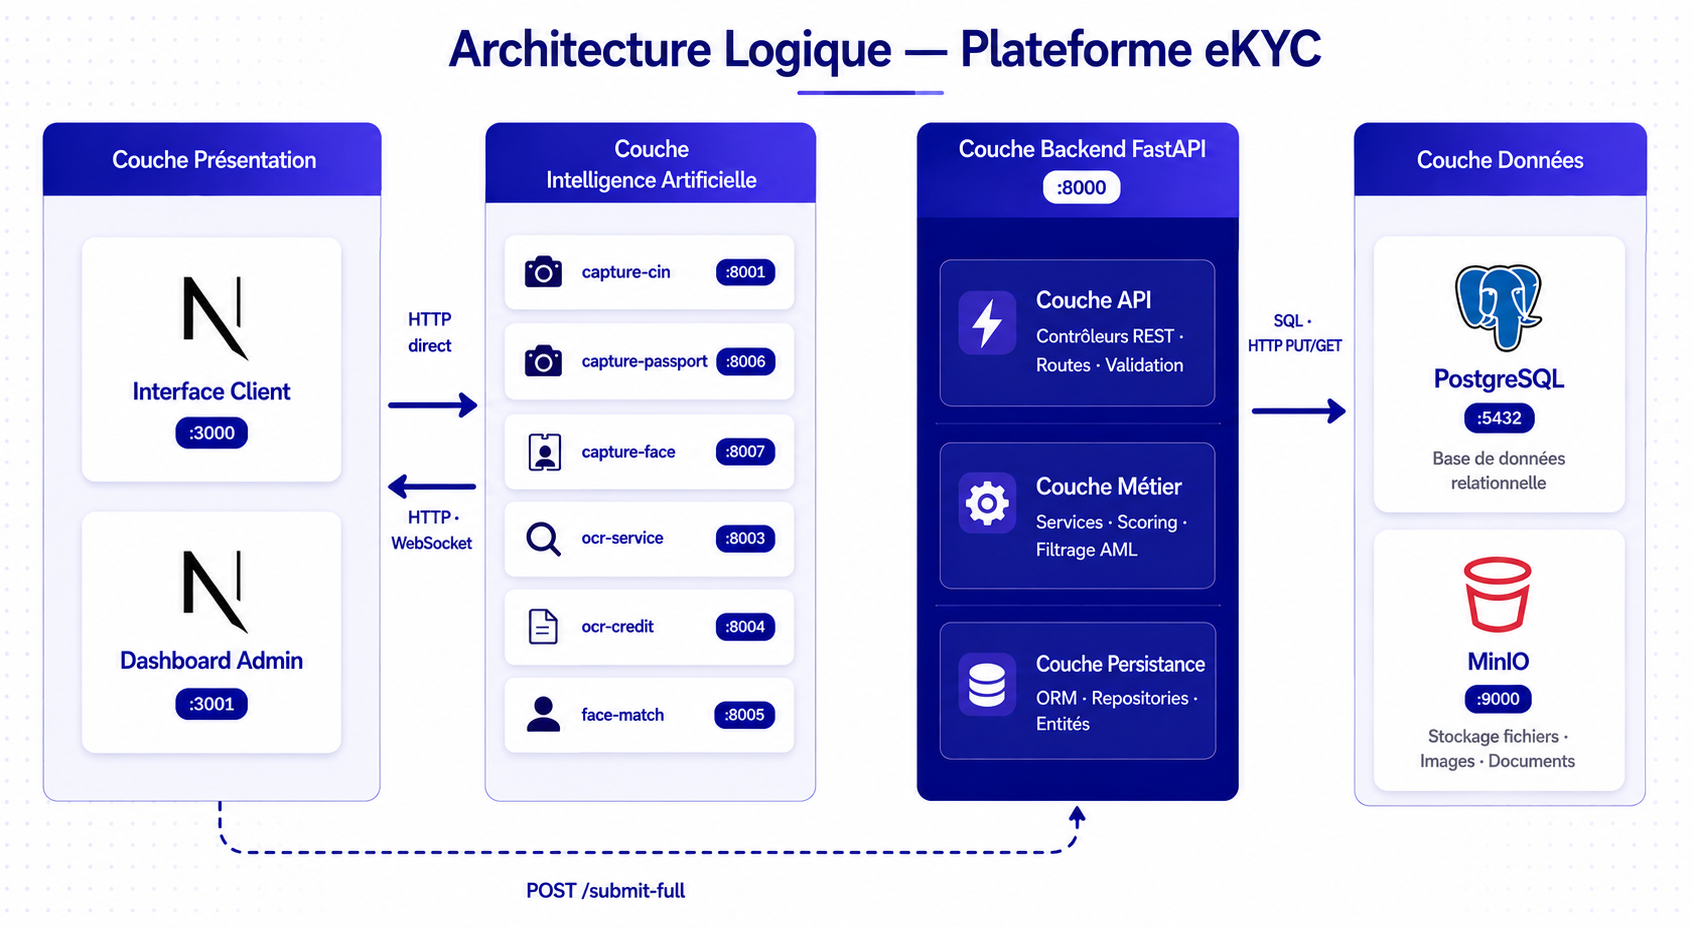
\includegraphics[width=0.95\textwidth]{images/architectures/logique.png}
  \captionof{figure}{Architecture logique de la plateforme eKYC}
  \label{fig:ch4-archi-logique}
\end{center}
\vspace{0.6em}

Cette organisation en quatre couches garantit une séparation claire des responsabilités. La vue physique ci-après précise comment ces couches se déploient concrètement sur l'infrastructure matérielle.

\subsection{Architecture physique}
\label{subsec:architecture-physique}

l'architecture physique de la plateforme eKYC, présentée dans la Figure~\ref{fig:ch4-archi-physique}, met en évidence les principaux éléments matériels et logiciels déployés ainsi que les échanges entre les postes clients, le serveur web, le serveur intelligence artificielle, le serveur backend et les serveurs de stockage. On y distingue les communications entre chaque composant : le poste client interagit avec le serveur web via HTTPS, le serveur web dialogue avec le serveur IA et le serveur backend, tandis que le serveur IA accède au stockage MinIO pour les images et le serveur backend persiste les données métier dans PostgreSQL.

\vspace{0.6em}
\begin{center}
  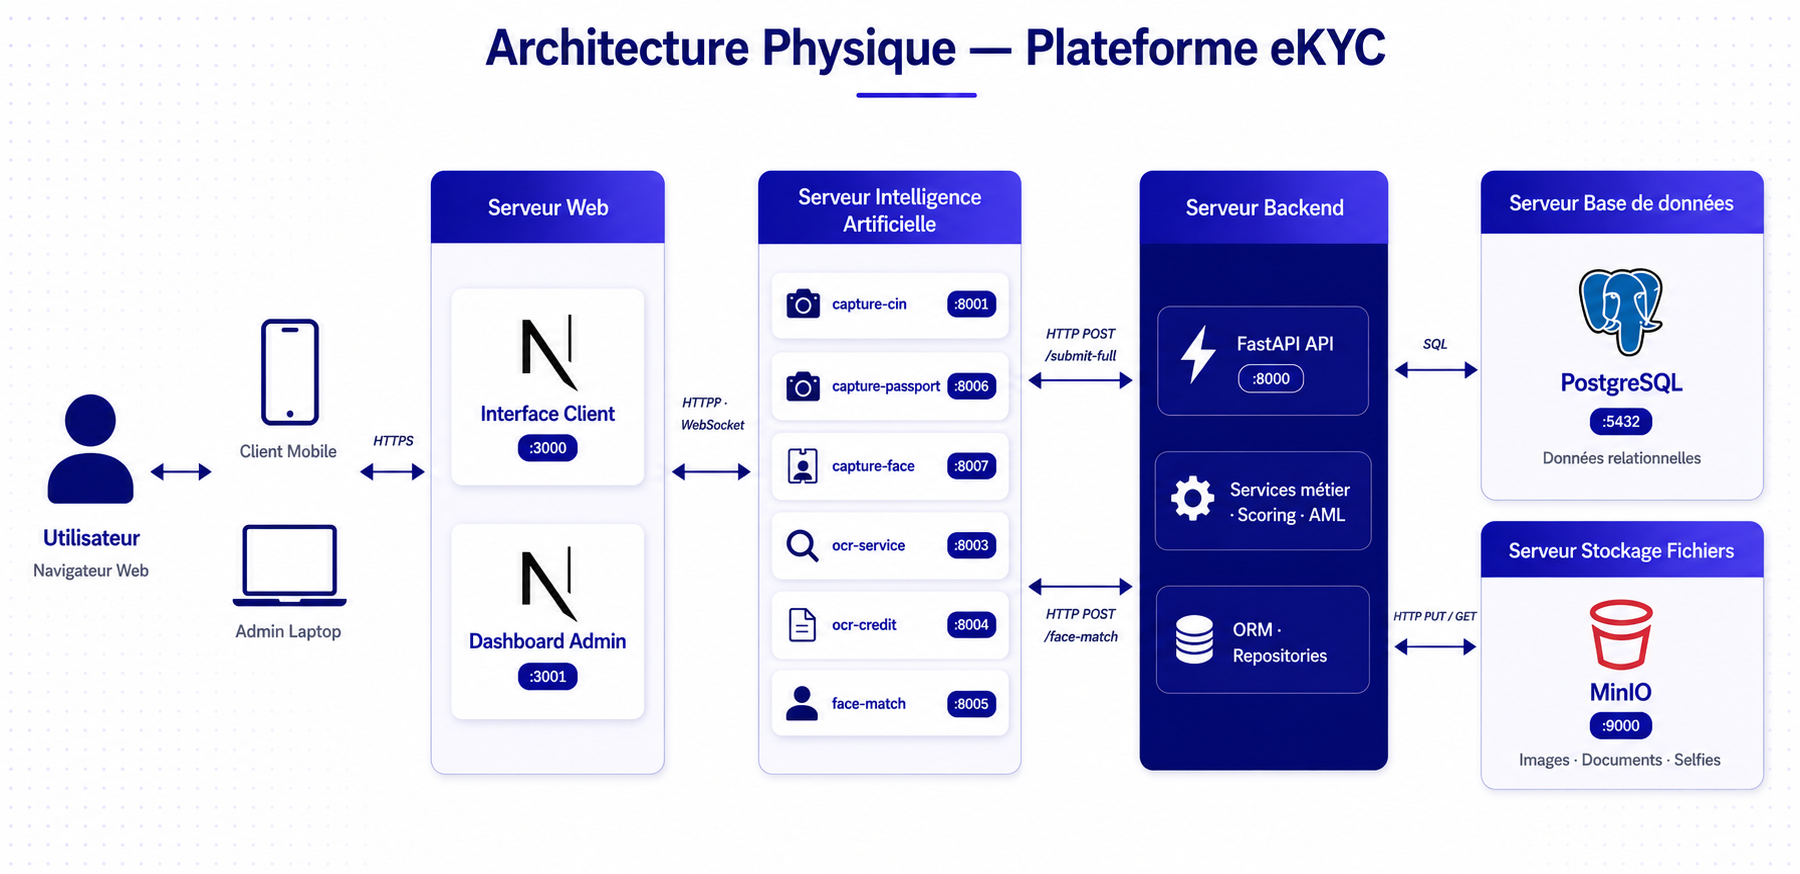
\includegraphics[width=0.95\textwidth]{images/architectures/physique.png}
  \captionof{figure}{Architecture physique de la plateforme eKYC}
  \label{fig:ch4-archi-physique}
\end{center}
\vspace{0.6em}

Les deux vues architecturales ainsi établies servent de base à la modélisation des interactions entre acteurs et système, formalisée dans la section suivante sous forme de diagrammes de cas d'utilisation.

%=============================================================
\section{Diagramme de cas d'utilisation global}
\label{sec:use-cases-global}
%=============================================================

Le diagramme de cas d'utilisation global illustrée par la Figure~\ref{fig:uc-global} offre une vue synthétique de l'ensemble des interactions entre les acteurs du système et la plateforme eKYC. Il met en évidence six profils d'acteurs aux périmètres fonctionnels distincts : le visiteur non inscrit, l'utilisateur authentifié engagé dans un parcours KYC, le client dont le compte est validé et qui accède aux services bancaires, l'analyste KYC chargé de statuer sur les dossiers, le responsable qualité IA qui surveille les performances des modèles, et l'administrateur qui hérite des droits des deux profils précédents tout en assurant la supervision globale de la plateforme.

\begin{figure}[H]
    \centering
    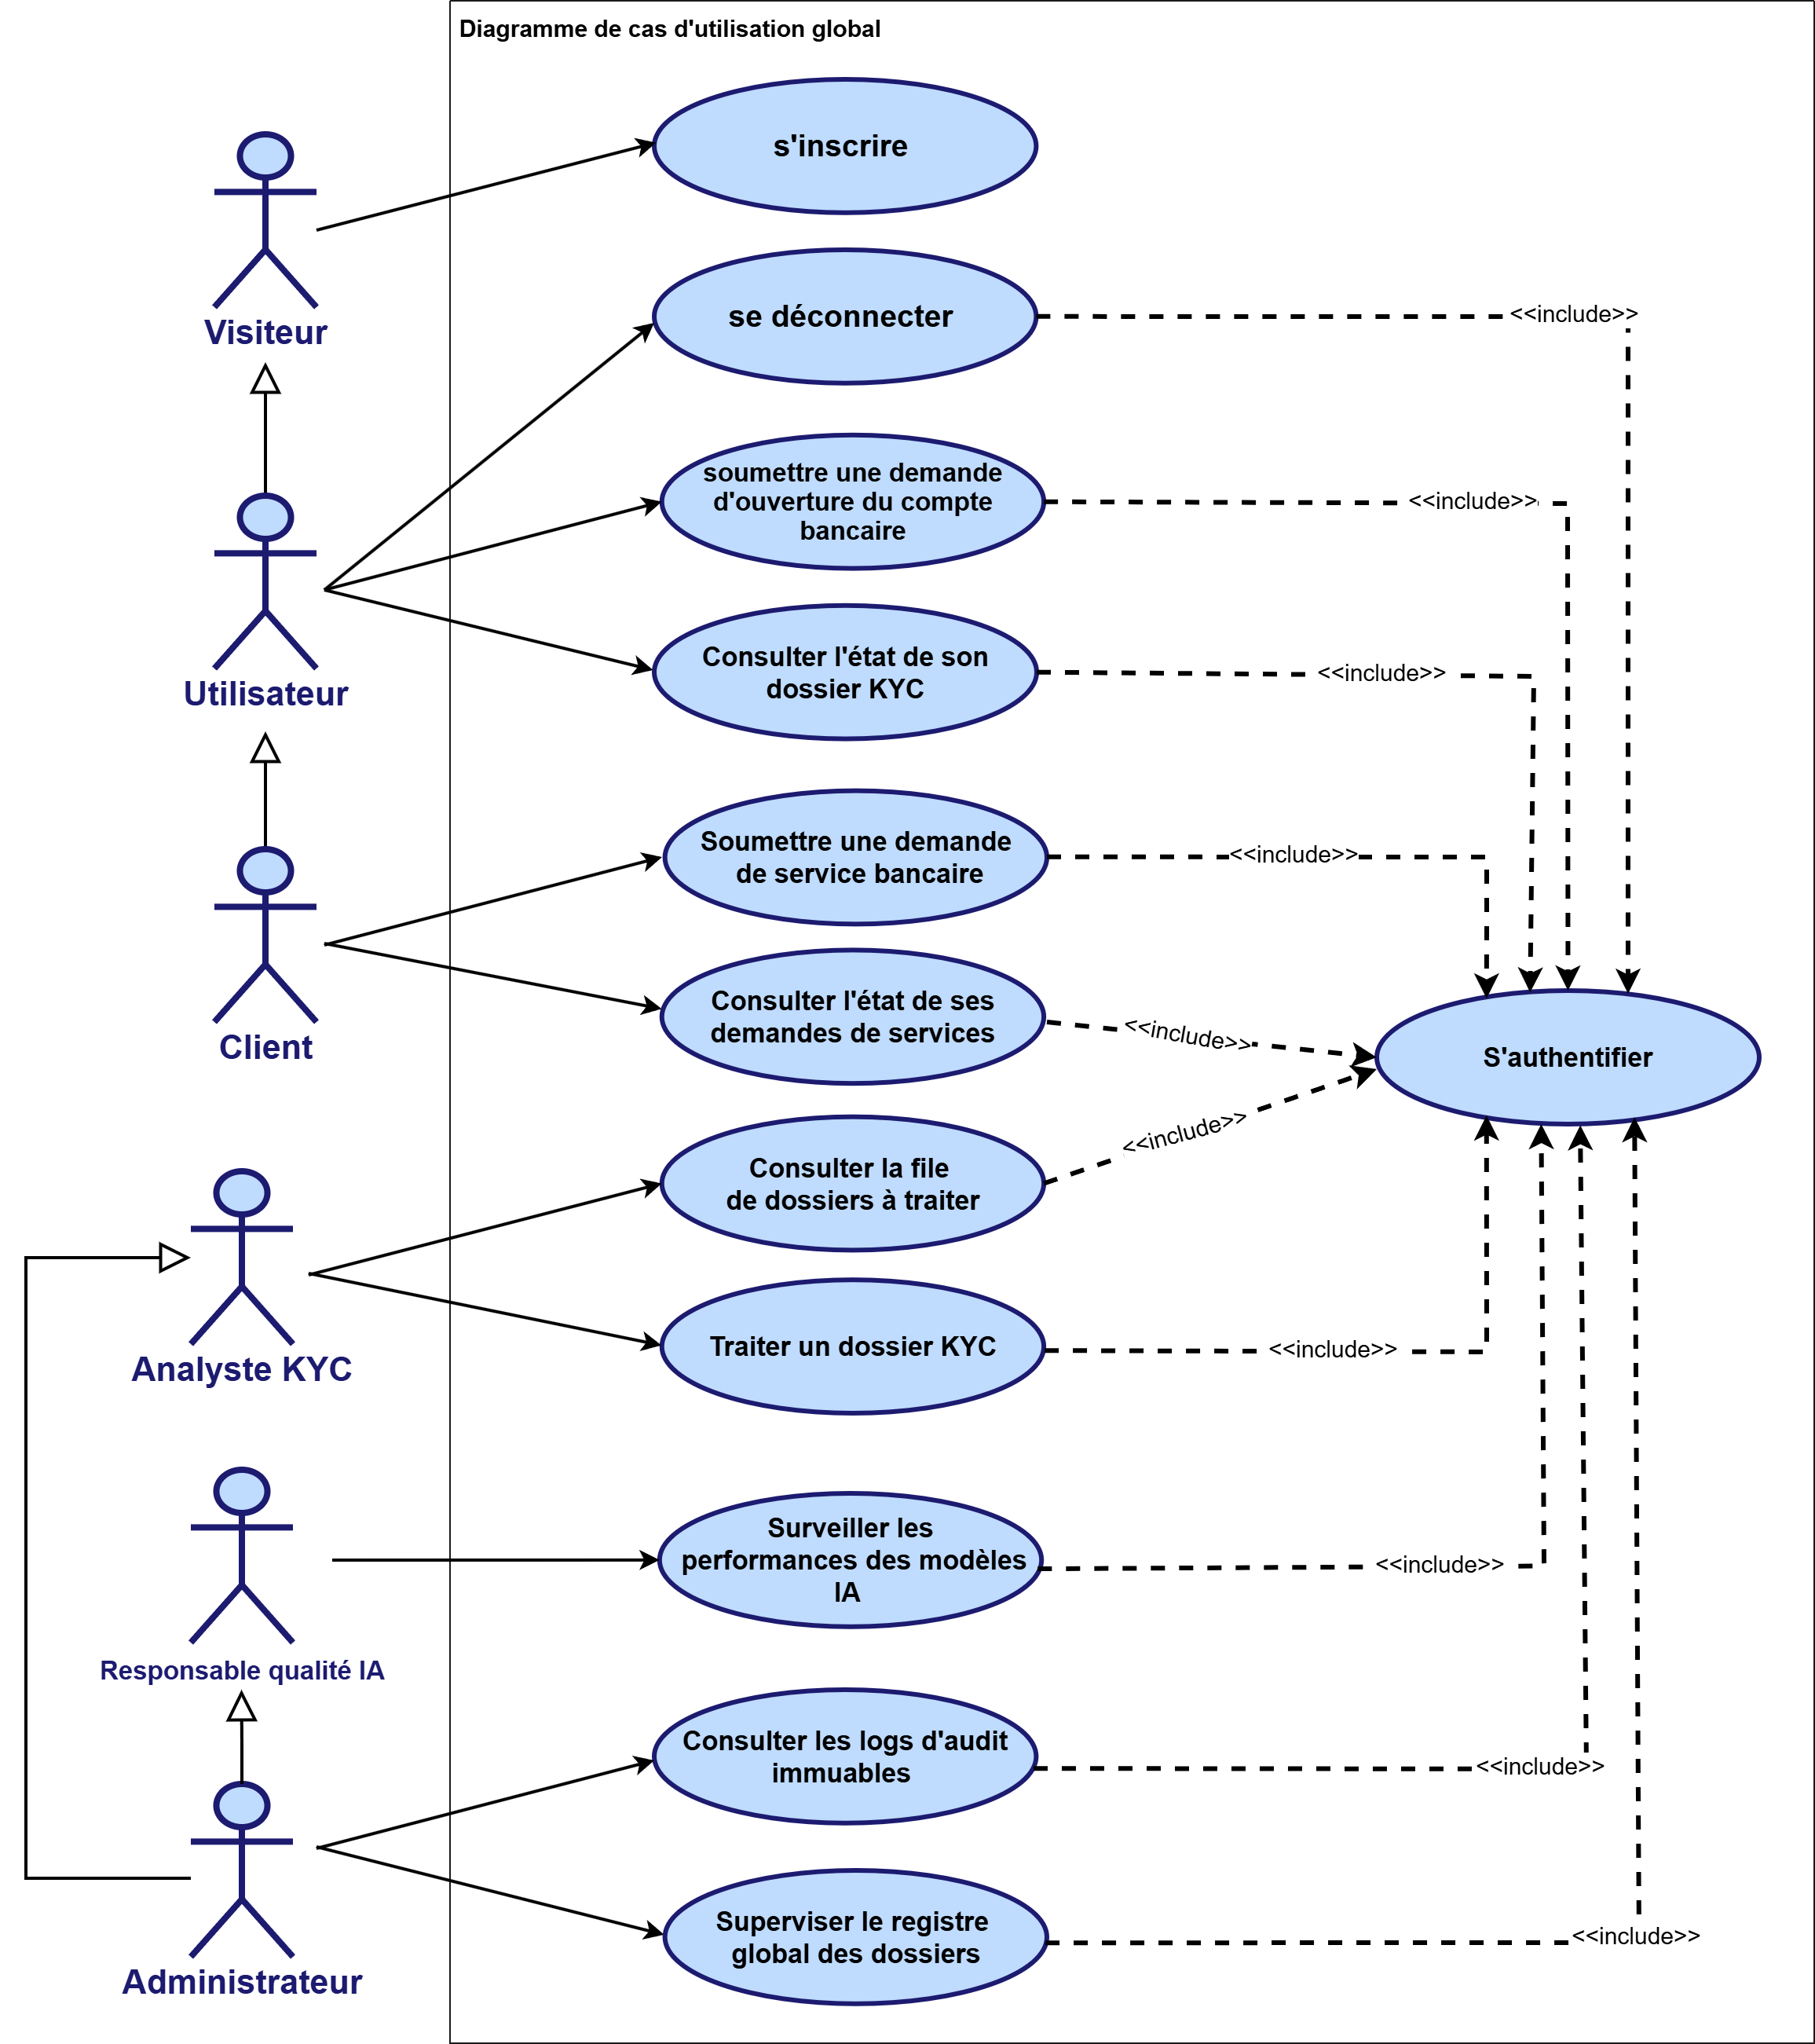
\includegraphics[width=\textwidth]{images/image_ch4/usecaseGlobale.png}
    \caption{Diagramme de cas d'utilisation global du système eKYC}
    \label{fig:uc-global}
\end{figure}

Ce diagramme constitue la vue d'ensemble des interactions du système. Les sous-sections suivantes détaillent chaque cas d'utilisation sous forme de tableaux structurés couvrant l'objectif, les préconditions, le scénario nominal et les alternatives.

%-------------------------------------------------------------
\subsection{Description des cas d'utilisation}
\label{subsec:description-uc}
%-------------------------------------------------------------

Les tableaux suivants décrivent de manière détaillée les principaux cas d'utilisation identifiés dans le diagramme global.

\renewcommand{\arraystretch}{1.5}

% ────────────────────────────────────────────────
% UC1 — S'inscrire
% ────────────────────────────────────────────────
\subsubsection{UC1 --- S'inscrire}

\begin{longtable}{|>{\bfseries}p{3.8cm}|p{10.2cm}|}
  \hline
  Cas d'utilisation    & S'inscrire (Création de compte) \\
  \hline
  Acteur principal     & Visiteur \\
  \hline
  Objectif             & Permettre à un visiteur de créer un compte sur l'interface client afin d'accéder au parcours KYC en utilisant son nom, son adresse électronique ou son numéro de téléphone et son mot de passe. \\
  \hline
  Préconditions        &
    - L'utilisateur ne possède pas encore de compte et accède à la page d'inscription. \newline
  \hline
  Scénario nominal     &
    - L'utilisateur accède au formulaire d'inscription de la plateforme. \newline
    - Il remplit le formulaire avec les informations requises : nom, adresse électronique ou numéro de téléphone et mot de passe. \newline
    - Le système valide les informations.\newline
    - Le système vérifie l'unicité de l'adresse électronique dans la base de données. \newline
    - Si toutes les informations sont valides, le compte est créé et un message de confirmation de création de compte est affiché. \newline
    - Le client est redirigé vers la page de connexion.. \\
  \hline
  Post-conditions      & Le compte de l'utilisateur est créé avec succès et enregistré dans la base de données. \\
  \hline
  Scénarios alternatifs &
    Le système affiche un message d'erreur et invite l'utilisateur à corriger les informations dans les cas suivants : \newline
    - Le format de l'adresse électronique est invalide ou le mot de passe est trop court. \newline
    - L'adresse électronique existe déjà dans la base de données (compte déjà existant). \\
  \hline
  \caption{UC1 --- S'inscrire}
  \label{tab:uc1}
\end{longtable}

Une fois le compte créé, l'utilisateur peut accéder à la plateforme via le mécanisme d'authentification décrit dans UC2.

% ────────────────────────────────────────────────
% UC2 — S'authentifier
% ────────────────────────────────────────────────
\subsubsection{UC2 --- S'authentifier}

\begin{longtable}{|>{\bfseries}p{3.8cm}|p{10.2cm}|}
  \hline
  Cas d'utilisation    & S'authentifier \\
  \hline
  Acteur principal     & Tout utilisateur disposant d'un compte (client, analyste KYC, responsable qualité IA, administrateur) \\
  \hline
  Objectif             & Accéder à l'espace personnel de la plateforme en présentant des identifiants valides. \\
  \hline
  Préconditions        &
    - L'utilisateur possède un compte actif sur la plateforme. \newline
    - L'utilisateur accède à la page de connexion. \\
  \hline
  Scénario nominal     &
    - L'utilisateur saisit son adresse électronique ou son numéro de téléphone(cas du client) et son mot de passe. \newline
    - Le système vérifie les identifiants et détermine le rôle associé au compte. \newline
    - L'utilisateur est redirigé vers l'interface correspondant à son profil (interface client, interface admin)\\
  \hline
  Post-conditions      & Une session sécurisée est ouverte. L'utilisateur accède aux fonctionnalités autorisées par son rôle. \\
  \hline
  Scénarios alternatifs &
    - Identifiants incorrects : le système affiche un message d'erreur générique sans préciser lequel des deux champs est erroné, par mesure de sécurité. \newline
    - Compte inexistant : l'utilisateur est invité à créer un compte ou à vérifier son adresse électronique. \\
  \hline
  \caption{UC2 --- S'authentifier}
  \label{tab:uc2}
\end{longtable}

Authentifié, l'utilisateur peut alors initier son parcours KYC, décrit dans UC3.

% ────────────────────────────────────────────────
% UC3 — Soumettre une demande KYC
% ────────────────────────────────────────────────
\subsubsection{UC3 --- Soumettre et suivre un dossier KYC}

\begin{longtable}{|>{\bfseries}p{3.8cm}|p{10.2cm}|}
  \hline
  Cas d'utilisation    & Soumettre et suivre un dossier KYC (parcours KYC) \\
  \hline
  Acteur principal     & Utilisateur authentifié \\
  \hline
  Objectif             & Déposer un dossier complet de demande d'ouverture de compte bancaire via un parcours guidé en quatre étapes, intégrant la capture du document d'identité, la vérification des données extraites, la capture du selfie biométrique et la soumission finale. \\
  \hline
  Préconditions        &
    - L'utilisateur est authentifié sur la plateforme. \newline
    - Il dispose d'un document d'identité valide (carte d'identité nationale ou passeport) et d'un accès à la caméra de son appareil. \\
  \hline
  Scénario nominal     &
    \textbf{Étape 1 : Capture du document d'identité.} L'utilisateur choisit le type de document (carte d'identité nationale en deux captures recto/verso, ou passeport en une seule capture). La caméra s'ouvre avec un cadre guide adapté. Le système analyse chaque image en temps réel~; le bouton de capture est initialement désactivé et ne s'active que lorsque le service IA confirme que le document détecté est valide (CIN ou passeport reconnu). L'utilisateur déclenche alors manuellement la capture. L'extraction des données textuelles est déclenchée en arrière-plan. \newline\newline
    \textbf{Étape 2 : Vérification des informations extraites.} L'utilisateur consulte les données extraites depuis son document. Il peut corriger manuellement tout champ inexact ; chaque correction est enregistrée et transmise à l'analyste KYC. \newline\newline
    \textbf{Étape 3 : Capture du selfie .} La caméra s'ouvre avec un cadre ovale centré. Le système détecte le visage en temps réel et active la capture dès que le cadrage est satisfaisant. \newline\newline
    \textbf{Étape 4 : Récapitulatif et soumission finale.} L'utilisateur vérifie l'ensemble des informations collectées, coche les cases de consentement et soumet sa demande. Le dossier complet est enregistré en base de données avec le statut « en attente » et un numéro de référence est communiqué à l'utilisateur. \\
  \hline
  Post-conditions      & Un dossier KYC complet est créé avec le statut « en attente ». L'utilisateur peut suivre l'évolution de son dossier depuis son espace personnel. \\
  \hline
  Scénarios alternatifs &
    - Document non reconnu : le système invite l'utilisateur à recommencer la capture dans de meilleures conditions d'éclairage. \newline
    - Selfie non conforme : l'utilisateur est invité à recommencer la capture en respectant les consignes de positionnement. \newline
    - Échec de soumission : les données restent conservées localement et l'utilisateur peut relancer la soumission. \\
  \hline
  \caption{UC3 --- Soumettre une demande d'ouverture de compte bancaire}
  \label{tab:uc3}
\end{longtable}

Une fois le dossier soumis par le client, il entre dans la file de traitement de l'analyste KYC, dont les actions sont formalisées dans UC4.

% ────────────────────────────────────────────────
% UC4 — Traiter un dossier KYC
% ────────────────────────────────────────────────
\subsubsection{UC4 --- Traiter un dossier KYC}

\begin{longtable}{|>{\bfseries}p{3.8cm}|p{10.2cm}|}
  \hline
  Cas d'utilisation    & Traiter un dossier KYC \\
  \hline
  Acteur principal     & Analyste KYC (ou Administrateur) \\
  \hline
  Objectif             & Examiner un dossier de demande d'ouverture de compte, vérifier la conformité des données et des documents soumis, et prendre une décision sur la suite à donner à la demande. \\
  \hline
  Préconditions        &
    - L'analyste est authentifié avec le rôle approprié. \newline
    - Au moins un dossier KYC est en attente de traitement dans la file. \\
  \hline
  Scénario nominal     &
    - L'analyste consulte la file d'attente des dossiers triée par ordre d'ancienneté et sélectionne un dossier à instruire. \newline
    - Il accède à la page de revue complète : images des documents, données extraites, corrections apportées par le client et résultat de la comparaison biométrique. \newline
    - Il vérifie les données extraites et corrige si nécessaire tout champ erroné. Chaque correction est horodatée et invalide les résultats de filtrage précédemment calculés. \newline
    - Le système présente les résultats de la vérification de conformité documentaire (cohérence des champs obligatoires, validité de la date d'expiration) et calcule un score de conformité. \newline
    - L'analyste lance le filtrage anti-blanchiment, qui confronte les données du client à la liste des personnes blacklistées, à la liste des personnes politiquement exposées et à la base des dossiers validés pour détecter d'éventuels doublons d'identité. \newline
    - L'analyste consulte le score de risque global agrégeant les résultats du filtrage, la conformité documentaire et la similarité biométrique. Le système formule une recommandation automatique. \newline
    - L'analyste prend sa décision finale : approbation, rejet motivé ou demande de complément documentaire. La décision est enregistrée et le client est notifié. \\
  \hline
  Post-conditions      & Le dossier est mis à jour avec la décision de l'analyste. Si approuvé, le compte bancaire est activé. Si rejeté, le motif est transmis au client. \\
  \hline
  Scénarios alternatifs &
    - Alerte AML confirmée : si l'alerte est avérée, la demande est rejetée ; si elle est écartée, le score de risque est recalculé en excluant cette alerte. \newline
    - Documents insuffisants : l'analyste sélectionne le statut « incomplet » et précise les pièces manquantes. \newline
    - Discordance biométrique : l'analyste peut rejeter la demande ou solliciter un complément d'information auprès du client. \\
  \hline
  \caption{UC4 --- Traiter un dossier KYC}
  \label{tab:uc4}
\end{longtable}

En parallèle du traitement des dossiers, le responsable qualité IA assure la supervision continue des modèles via UC5.

% ────────────────────────────────────────────────
% UC5 — Surveiller les performances des modèles IA
% ────────────────────────────────────────────────
\subsubsection{UC5 --- Surveiller les performances des modèles IA}

\begin{longtable}{|>{\bfseries}p{3.8cm}|p{10.2cm}|}
  \hline
  Cas d'utilisation    & Surveiller les performances des modèles IA \\
  \hline
  Acteur principal     & Responsable qualité IA (ou Administrateur) \\
  \hline
  Objectif             & Évaluer en continu la qualité des traitements automatiques produits par les modèles de détection et d'extraction, afin de détecter toute dégradation de performance et d'orienter les actions correctives. \\
  \hline
  Préconditions        &
    - Le responsable est authentifié avec le rôle approprié. \newline
    - Des dossiers ont été traités par le système, générant des données de performance exploitables. \\
  \hline
  Scénario nominal     &
    - Le responsable accède à la page de supervision IA et sélectionne le type de document à analyser (carte d'identité recto, verso ou passeport) ainsi que la période d'observation. \newline
    - Il consulte les indicateurs clés de performance globaux : précision, rappel, score F1 et latence moyenne pour le pipeline complet et pour chacun des deux modèles séparément. \newline
    - Il examine le graphique d'évolution hebdomadaire des scores de confiance pour détecter toute tendance à la dégradation dans le temps. \newline
    - Il analyse les performances du modèle de détection champ par champ : score de confiance moyen, taux de zones manquantes et taux de faux positifs. \newline
    - Il analyse les performances du moteur de lecture champ par champ : score de confiance OCR moyen, taux de corrections manuelles et taux de champs vides. \newline
    - Il consulte le graphique de corrélation entre les scores des deux modèles pour identifier les zones présentant une incohérence. \newline
    - En cas d'anomalie, il documente ses observations et déclenche une action corrective sur le modèle ou le prétraitement concerné. \\
  \hline
  Post-conditions      & Le responsable dispose d'une vue objective et actualisée de la qualité des traitements. Les anomalies identifiées sont documentées et transmises aux équipes techniques. \\
  \hline
  Scénarios alternatifs &
    - Dégradation détectée : un signal d'alerte visuel est affiché lorsqu'un indicateur passe sous le seuil de qualité cible (ex. taux de correction dépassant 10\,\% sur un champ). \newline
    - Aucune donnée disponible : la page affiche un message informatif et invite à élargir la fenêtre temporelle d'observation. \\
  \hline
  \caption{UC5 --- Surveiller les performances des modèles IA}
  \label{tab:uc5}
\end{longtable}
\section*{Conclusion du chapitre}

Ce chapitre a établi le référentiel complet de la plateforme eKYC : identification des quatre profils d'acteurs, formalisation des besoins fonctionnels couvrant l'ensemble du parcours client et des fonctions d'administration, et définition des contraintes non fonctionnelles en matière de sécurité, de confidentialité, de conformité réglementaire et de performance. L'architecture logique et physique retenue traduit ces exigences en une organisation modulaire et souveraine, tandis que les diagrammes de cas d'utilisation en formalisent les interactions. Ces éléments constituent le socle sur lequel s'appuient la conception détaillée et la réalisation présentées dans les chapitres suivants.
